\section{Nerozlišitelné částice}
    \subsection{Kvantový tlak}
        Určete střední energii jedné částice nerelativistického fermionového plynu o hustotě počtu částic $\rho$.
        Určete, jaký je v tomto plynu tlak.

    \subsection{Relativistický kvantový tlak}
        Zopakujte řešení předchozí úlohy pro ultrarelativistický fermionový plyn (rychlosti částic plynu jsou tak velké, že lze zanedbat jejich klidovou hmotnost).

    \subsection{Poloměr hvězdy}
        Odhadněte poloměr vyhořelé hvězdy (bílého trpaslíka) s hmotností $M$.
        Předpokládejte, že hvězda je složena z uhlíků $^{12}$C.

    \subsection{Chandrasekharova mez}
        Odhadněte Chandrasekharovu mez pro bílého trpaslíka (jedná se o mezní hmotnost, nad kterou již kvantový tlak neudrží hvězdu proti gravitační síle a hvězda se zhroutí do neutronové hvězdy nebo černé díry).

    \subsection{Interakce způsobená nerozlišitelností volných částic}
        Uvažujte dvě nerozlišitelné volné částice o hmotnosti $m$ pohybující se na přímce.
        Jejich vlnové funkce jsou dány gaussovskými balíky dobře lokalizovanými okolo bodů $-b$ a $+b$ (obrázek),
        \begin{equation}
            \psi_{\pm}(x)=\frac{1}{\sqrt[4]{\pi\sigma^{2}}}\e^{-\frac{1}{2\sigma^{2}}(x\mp b)^{2}},
        \end{equation}
        kde $\sigma\ll b$ určuje určuje šířku balíku.
        
        \begin{figure}[htbp!]
            \centering
            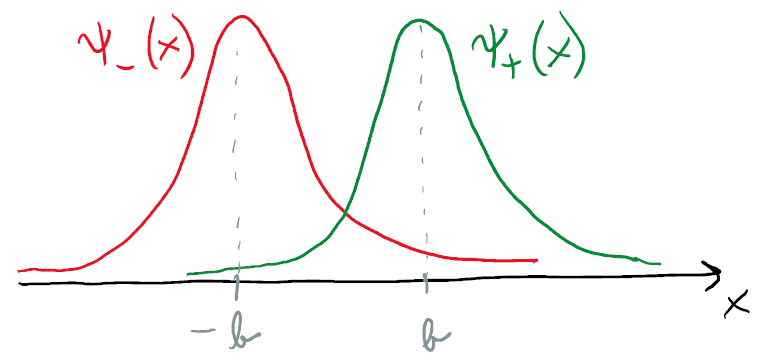
\includegraphics[width=0.5\linewidth]{Identical.png}
        \end{figure}

        \begin{enumerate}
            \item 
                Určete vlnovou funkci $\psi(x_{1},x_{2})$ systému těchto dvou nerozlišitelných částic a spočítejte její normalizaci.
                Vlnové funkce mohou být symetrické (bosony, fermiony s antisymetrickým spinovým stavem) nebo antisymetrické (fermiony se symetrickým spinovým stavem). 
                Uvažujte oba dva případy.
            
            \item Spočítejte střední hodnotu energie systému dvou nerozlišitelných částic
                \begin{equation}
                    E=\matrixelement{\psi}{\operator{H}}{\psi}=\int\psi^{*}(x_{1},x_{2})H\psi(x_{1},x_{2})\d x_{1}\d x_{2}.
                \end{equation}

            \item Spočítejte efektivní sílu
                \begin{equation}
                    F\equiv-\frac{\partial E}{\partial b}.
                \end{equation}
                Bude tato síla přitažlivá nebo odpudivá a jak závisí na symetrii vlnové funkce?
        \end{enumerate}
